\documentclass{article}
\usepackage[utf8]{inputenc}
\usepackage{hyperref}
\usepackage{amsmath}
\usepackage{amsfonts}
\usepackage{graphicx}
\usepackage{enumitem}
\graphicspath{ {./images} }


\title{Freshman Physics}
\author{
    Tan Chien Hao\\
    \texttt{www.tchlabs.net}\\
    \texttt{Telegram @tch1001}
    % new collaborators add your name and contact here!
}

\date{\today}
\begin{document}

\maketitle
\tableofcontents

\section{Math: Functions}
Functions are maps from one set to another set. We denote them as $f: A \rightarrow B$ or $f(x) \in B$ where $x\in A$. \\
\\
Examples of functions $f: \mathbb R \to \mathbb R$:
\begin{itemize}
    \item Particle's x coordinate $x(t) = 5 \sin (2t)$
    \item Particle's x component of velocity $v_x(t) = 10 \cos (2t)$
    \item Particle's x component of acceleration $a_x(t) = - 20 \sin (2t)$
    \item Potential Energy of spring mass system $U(x) = \frac{1}{2} k(x-x_0)^2$
    \item Current flowing through Resistor Capacitor circuit $I(t) = I_0 e^{-{t}/{RC}}$
    \item Kinetic Energy in terms of speed $T(|\vec{v}|) = \frac{1}{2} m |\vec{v}|^2$
\end{itemize}
\leavevmode \\
Examples of functions $f: \mathbb R \to \mathbb R^3$:
\begin{itemize}
    \item Particle path in 3D $\vec{s}(t) = \left(\begin{array}{l}
         x(t) \\
         y(t) \\
         z(t) 
    \end{array}\right) $
\end{itemize}
\leavevmode \\
Examples of functions $f: \mathbb R^3 \to \mathbb R$:

\begin{itemize}
    \item Gravitational Potential $\phi(x,y,z) = -\frac{GM}{\sqrt{x^2+y^2+z^2}}$
    \item Electric Potential Energy $\phi(\vec{r}) = -\frac{kQq}{|\vec{r}|}$. The arrow above $\vec{r}$ means it is a vector (more on this later)
    \item Temperature $T(\vec{r})$
\end{itemize}
\leavevmode \\
Examples of functions $f: \mathbb R^3 \to \mathbb R^3$:

\begin{itemize}
    \item Gravitational Force $\vec{F}(x,y,z) = -\frac{GMm}{(x^2 + y^2 + z^2)^{3/2}} \left(\begin{array}{l}
x \\
y \\ 
z
\end{array}\right)$
    \item Electrostatic Force $\vec{F}(\vec{r}) = \frac{kQq}{|\vec{r}|^2} \hat{r}$. The hat above $\hat{r}$ means it is a unit vector (scaled $\vec{r}$ to have length $1$).
\end{itemize}

\section{Math: Differentiation}
You probably know how to calculate the gradient of a linear (aka straight) graph.
$$m = \frac{y_1 - y_0}{x_1 - x_0}$$
This works if the graph is linear, i.e. $y=mx+c$. But what happens if the graph is not linear? e.g. $y = x^2$. How can we calculate the gradient of this curvy graph? Answer is \textbf{Differentiation}.

(Most) functions can be differentiated \textbf{with respect to} their parameters. \textbf{Algebraically}, differentiation involves following a set of rules. \textbf{Geometrically}, differentiation is the slope of the tangent line to the function's graph. 

\subsection{Geometric Intuition}
\url{https://www.desmos.com/calculator/b6ts3ls1zf} Desmos visualization. Given a function $f(x)$, here's what the derivative $\frac{d}{dx}f = \frac{df}{dx} = f'(x)$ means:
\begin{itemize}
    \item Draw the graph $y=f(x)$.
    \item For each $x = x_0$ value, find the point on the graph $(x_0,f(x_0))$.
    \item Draw a (straight) tangent line to the graph at that point.
    \item Calculate the gradient of that tangent line.
    \item This gradient is the "derivative of $f$ \textbf{at }$x=x_0$".
    \item If you chose a different $x=x_1$ value, you would get a different value for gradient, and that would be "derivative of $f$ \textbf{at }$\mathbf{x=x_1}$".
    \item So the derivative of a function $f(x)$ is another function $f'(x)$.
\end{itemize}

\subsubsection{Finding Maximum / Minimum}
When the function $f(x)$ has a maximum $x_{\text{max}}$, the derivative at that maximum point is zero $$\left. \frac{df}{dx} \right|_{x_{\text{max}}} = 0$$
Likewise for minimum.\\[10pt]
So if the function has $0$ derivative at some $x=x_0$, how do we determine if it's a maximum or minimum point? We can perform the 2nd derivative test.\\

\begin{align}
    \left. \frac{d^2 f}{dx^2} \right|_{x_0} > 0 &: \text{Minimum}\\
    \left. \frac{d^2 f}{dx^2} \right|_{x_0} < 0 &: \text{Maximum}\\
    \left. \frac{d^2 f}{dx^2} \right|_{x_0} = 0 &: \text{Not enough information to conclude}
\end{align}

\subsection{Algebraic Calculations}
From the above geometric explanation, one can calculate the derivative of $f(x) = x^2$ to be $f'(x) = 2x$. This method of differentiation is called "from first principles".
\begin{align*}
f^{\prime}(x) & =\lim _{h \rightarrow 0} \frac{f(x+h)-f(x)}{h} \\
& =\lim _{h \rightarrow 0} \frac{\left((x+h)^2\right)-\left(x^2\right)}{h} \\
& =\lim _{h \rightarrow 0} \frac{x^2+2 h x+h^2-x^2}{h} \\
& =\lim _{h \rightarrow 0} \frac{2 h x+h^2}{h} \\
& =\lim _{h \rightarrow 0} \frac{h(2 x+h)}{h} \\
& =\lim _{h \rightarrow 0} 2 x+h \\
& =2 x
\end{align*}

One can use first principles to derive the following rules of differentiation for common functions:

\begin{itemize}
    \item Linearity (Adding) 
    \begin{align}
        \frac{d}{dx} [f(x) + g(x)] &= \frac{df}{dx} + \frac{dg}{dx} \\
    \frac{d}{dx} [c f(x)] &= c \frac{df}{dx}
    \end{align}
    \item Polynomial $$ \frac{d}{dx} x^n = nx^{n-1} $$
    \item Trigonometry \begin{align}
        \frac{d}{dx} \sin(x) & = \cos(x) \\
        \frac{d}{dx} \cos(x) & = -\sin(x)
    \end{align}
    \item Exponential $$\frac{d}{dx} e^x = e^x$$
    \item Product Rule $$\frac{d}{dx} [f(x) g(x)] = f(x) \frac{dg}{dx} + g(x) \frac{df}{dx}$$
    \item Chain Rule $$\frac{d}{dx} f(y(x)) = \frac{df}{dy} \frac{dy}{dx}$$
\end{itemize}

\subsection{Exercises}
Try differentiating the following functions with respect to $x$ or $t$. You can check your answer against Wolfram Derivative Calculator \url{https://www.wolframalpha.com/calculators/derivative-calculator/}.

\begin{itemize}
    \item $\frac{d}{dx} x^4 + x^2$
    \item $\frac{d}{dt} 5t + 3$
    \item $\frac{d}{dx} \frac{1}{x}$
    \item $\frac{d}{dt} \sin (2t)$
    \item $\frac{d}{dt} e^{-5t}$
    \item $\frac{d}{dx} \tan x$
\end{itemize}

\section{Math: Integration / Anti-Differentiation (Basic)}

Geometrically, (definite) integration gives you the area under the graph. Algebraically, there are a few techniques for common functions but integration is tricky in general. 

\subsubsection{Indefinite Integration / Antiderivative}
Q: If I give you a function $f(x)$ and told you that it's derivative is $f'(x) = 2x + 1$, can you find out what $f(x)$ is? \\
A: $f(x) = x^2 + x + C$ where $C$ is an arbitrary constant. Why are there multiple answers?

Mathematically, we say $$\int 2x + 1\ dx = x^2 + x + C$$
More generally, $$\int f'(x) dx = f(x) + C$$

\subsubsection{Exercises}
You can check whether you are correct by putting your answer in the derivative calculator and checking if you get the function to be integrated!
\begin{itemize}
    \item $\int 5\ dx$
    \item $\int \left( \int -10 dt \right) dt$
    \item $\int \sin(5t) \ dt$
    \item $\int (1/x^2) dx$
\end{itemize}


\textbf{Extra:} Some functions have antiderivatives that cannot be even expressed analytically, such as $$\int e^{-x^2} dx$$

\subsubsection{Definite Integration / Area under graph}
You can calculate the area under a curve by performing a \textbf{definite} integral.
\begin{align}
    \text{Area under }f'(x)\text{ from }x=a\text{ to }x=b &= \int_a^b f'(x)\ dx  \\
    &= \left[f(x) + C\right]^b_a \\
    &= f(b) - f(a)
\end{align}

Q: Why does the arbitrary constant $C$ not appear in the formula for area under the graph? 

A: It cancels out: $[f(b) + C] - [f(a) + C]$. Can you imagine this graphically? 

\subsubsection{Exercises}

\begin{itemize}
    \item Energy in Spring
        $$\int_0^x kr\ dr$$
    \item Energy in Capacitor
        $$\int_0^Q \frac{q}{C} dq$$
    \item Gravitational Potential
        $$\int_{r}^{\infty} \frac{1}{x^2} dx$$
\end{itemize}

\section{Physics: Kinematics}

After picking a direction which you define as "increasing x direction" as well as an origin for x, you can start describing 1D motion $x(t)$.\\
\\
If you want to describe 2D motion, pick a perpendicular y-axis. \\
\\
If you want to describe 3D motion, z-axis is defined using RHR (for the cross product).
\subsection{Path of Particle / Object}
Mathematically, paths are functions $\vec{s}(t)$ of a parameter $t$ representing time. 
\begin{itemize}
    \item In 1D motion, $x(t)$ 
    \item In 2D motion, $x(t),\ y(t)$
    \item In 3D motion, $x(t),\ y(t),\ z(t)$
\end{itemize}
To understand an object's behaviour, our goal is to solve for the 3 functions $x(t),\ y(t),\ z(t)$, meaning we obtain a formula like $y(t) = 2 t - 5 t^2$. Knowing where the object is at every snapshot in time allows us to calculate it's velocity $\vec{v}(t)$, it's acceleration $\vec{a}(t)$, how long it'll take to travel from A to B ($\Delta t = t_B - t_A$), the forces $\vec{F}(\vec{s}(t))$ acting on it at any time, etc.

\subsection{SUVAT}
\begin{align}
v(t)&=u+a t \label{eq:vuat} \\
s(t)&=u t+\frac{1}{2} a t^2 \label{eq:suat}\\
 v(s)^2&=u^2+2 a s \label{eq:vuas} \\
 s(t)&=\frac{v(t)+u}{2} t \label{eq:svut}\\
 s(t)&=v(t) t-\frac{1}{2} a t^2 \label{eq:svat}
\end{align}
SUVAT laws can be derived from calculus with the following definitions.\\[10pt]
Let $s(t)$ be the function representing the particle's (1D) coordinate.
\begin{align}
    v(t) &:= \frac{ds}{dt} \\
    a(t) &:= \frac{dv}{dt} = \frac{d^2 s}{dt^2}
\end{align}
\\
If acceleration is constant, i.e. $$a(t) = \frac{d^2 s}{dt^2} = a_0$$ for some constant $a_0$, then one can integrate the above equation once and twice to get 2 of the SUVAT laws 

\begin{align}
    v(t) &= a_0 t + v_0 \\
    s(t) &= \frac{1}{2} a_0 t^2 + v_0 t + s_0 
\end{align}
\\
where we identify $a_0 \equiv a$, $v_0 \equiv u$, $s_0 \equiv 0$ to match \ref{eq:vuat} and \ref{eq:suat}.\\
\\
The other 3 equations can be obtained from the first 2 with a bit of algebra.\\

\subsection{Geometric Intuition}
SUVAT can be visualized as an area of a trapezium in the $v\text{-}t$ graph. [Demonstrate in class]


\subsection{Exercises}
\begin{samepage}
    
SJPO 2015 General Round Q13: An object is travelling on a straight path and exhibiting a constant acceleration $a$ starts off with an initial velocity $v=2.0 \mathrm{~ms}^{-1}$. It has traversed $4.5 \mathrm{~m}$ in the third second (from $t=2$ to $t=3$), its acceleration $a$ is
\begin{itemize}\item[](A) $0.5 \mathrm{~ms}^{-2}$
 \item[](B) $1.0 \mathrm{~ms}^{-2}$
\item[](C) $1.5 \mathrm{~ms}^{-2}$
\item[](D) $2.0 \mathrm{~ms}^{-2}$
\item[](E) $2.5 \mathrm{~ms}^{-2}$
\end{itemize}
Ans: B
\end{samepage}
\\[20pt]
% SJPO 2015 General Round Q28: The Moon is approximately $380,000 \mathrm{~km}$ from Earth. The time a laser light beam takes to travel from the Earth to the Moon and back is most nearly
% \begin{itemize}\item[](A) 2 microseconds.
% \item[](B) 2 milliseconds.
% \item[](C) 2 seconds.
% \item[](D) 2 minutes.
% \item[](E) 2 hours. 
% Ans:C
\begin{samepage}
\subsubsection{SJPO 2016 General Round Q8}
A train moving on straight horizontal tracks slows down from $66 \mathrm{~ms}^{-1}$ to $22 \mathrm{~ms}^{-1}$ at a constant rate of $2.0 \mathrm{~ms}^{-2}$. What distance does it travel while slowing down?
\begin{itemize}
\item[](A) $490 \mathrm{~m}$
\item[](B) $650 \mathrm{~m}$
\item[](C) $740 \mathrm{~m}$
\item[](D) $970 \mathrm{~m}$ 
\item[](E) $1100 \mathrm{~m}$ \end{itemize}
Ans: D
\end{samepage}
\\[20pt]
% SJPO 2016 General Round Q9 A (Projectile Motion)
% SJPO 2016 General Round Q11 E (Projectile)
\begin{samepage}
\subsubsection{SJPO 2018 General Round Q10} The position of an object moving along a linear track is plotted as a function of time. It started from rest and underwent a positive acceleration for some time, followed by a constant velocity. Which of the following graphs correctly shows this situation?\\
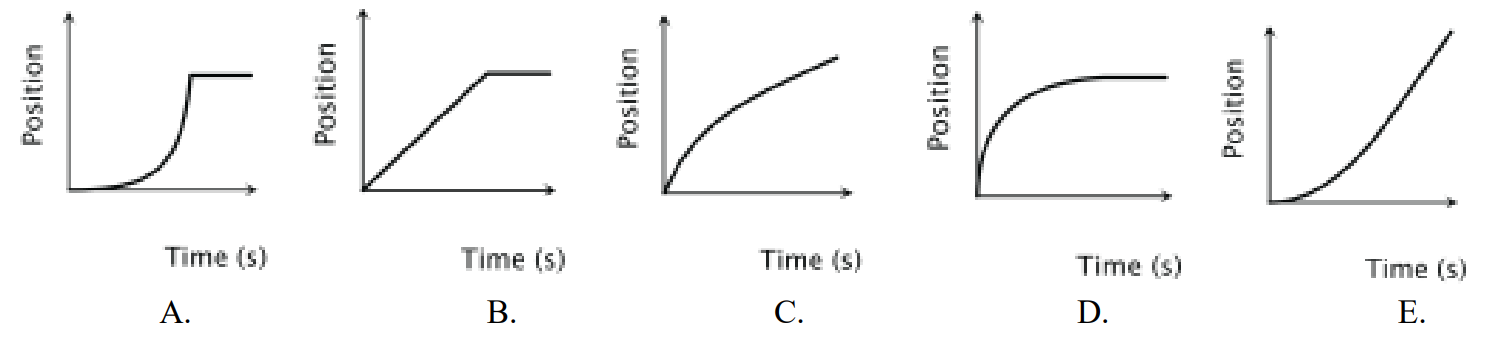
\includegraphics[width=\linewidth]{2018q10.png}\\
Ans: E\\
\end{samepage}
% SJPO 2018 General Round Q11 B
% SJPO 2018 General Round Q13 A
\subsubsection{SJPO 2018 General Round Q16 \& Q17}
A car travels along a straight road with the speed shown by the 
v-t graph. \\ 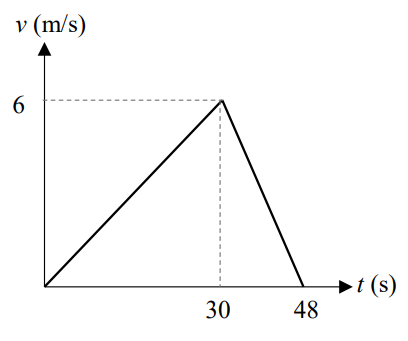
\includegraphics[width=0.5\linewidth]{images/2018q16.png} \\
\\
\begin{samepage}
16. What is the acceleration of the car from $t=30$ to $t=48 \mathrm{~s}$ ?
\begin{itemize}
\item[] (A) $-54 \mathrm{~m} / \mathrm{s}^2$ 
\item[] (B) $\quad 48 \mathrm{~m} / \mathrm{s}^2$ 
\item[] (C) $-3.0 \mathrm{~m} / \mathrm{s}^2$ 
\item[] (D) $\quad 3.0 \mathrm{~m} / \mathrm{s}^2$
\item[] (E) $-0.33 \mathrm{~m} / \mathrm{s}^2$\end{itemize}
Ans: E
\end{samepage}
\\[20pt]
\begin{samepage}
17. What is the total displacement of the car after $48 \mathrm{~s}$ ?
\begin{itemize}
\item[] (A) $36 \mathrm{~m}$
\item[] (B) $48 \mathrm{~m}$
\item[] (C) $144 \mathrm{~m}$
\item[] (D) $180 \mathrm{~m}$
\item[] (E) $210 \mathrm{~m}$ 
\end{itemize}
Ans: C\\
\end{samepage}
\\
\begin{samepage}
\subsubsection{SJPO 2017 General Round Q1} 
An electron in a vacuum, starting from rest falls $5 \mathrm{~cm}$ near the surface of the earth. Considering only the gravitational force acting on the electron, how long does it take for the electron to travel $5 \mathrm{~cm}$?
\begin{itemize}
\item[] (A) $\quad 0.1 \mathrm{~s}$
\item[] (B) $\quad 0.03 \mathrm{~s}$
\item[] (C) $\quad 0.01 \mathrm{~s}$
\item[] (D) $\quad 0.001 \mathrm{~s}$
\item[] (E) $\quad 0.0001 \mathrm{~s}$
\end{itemize}
Ans: A
\end{samepage}
% SJPO 2018 General Round Q18 C

\subsection{1D Dynamics}
If we know the acceleration as a function of time $a(t)$, as well as the initial velocity $v(t=0) \equiv v_0$ and position $s(t=0) \equiv s_0$, then we can integrate $a(t)$ twice to get the position as a function of time 
$$s(t) = \int \left(\int a(t)\ dt\right)\ dt$$

To obtain this $a(t)$, we use Newton's 2nd law 
$$F_{\text{net}}(t) = \frac{d(mv)}{dt} = m \frac{dv}{dt} + v \frac{dm}{dt}$$
In (most) cases where $m(t)$ is a constant wrt time, 
$$F_{\text{net}}(t) = ma(t)$$



\subsection{Extra: $v^2 = u^2 + 2as$ Connection with Work Energy Theorem}
$v^2 = u^2 + 2as$ is slightly special because it is related to "work energy theorem" in dynamics. One can derive it by integrating $a(t)$ wrt $s(t)$ instead of $t$ 
\begin{align}
    \frac{d^2 s}{dt^2} &= a_0 \\
    \frac{d}{dt} \left(\frac{ds}{dt}\right) \frac{ds}{dt} dt &= a_0 ds \\
    \frac{1}{2} \frac{d}{dt} \left( v(t)^2 \right) dt &= a_0 ds \\
    \int_{t_A}^{t_B} \frac{1}{2} \frac{d}{dt} \left( v(t)^2 \right) dt &= \int_{s_A}^{s_B} a_0 ds \\
    \int_{v_A}^{v_B} \frac{1}{2} d\left( v^2 \right) &= a_0 (s_B - s_A) \\
    \frac{1}{2} (v_B^2 - v_A^2) &= a_0 (s_B - s_A) \\
    v_B^2 &= v_A^2 + 2a_0(s_B - s_A)
\end{align}

where we identify $v_B \equiv v$, $v_A \equiv u$, $s_B \equiv s$, $s_A \equiv 0$, $a_0 \equiv a$ to match \ref{eq:vuas}.
\\
 
\textbf{Extra:} If the function of \textbf{multiple variables} is differentiated, it's called \textbf{multivariate calculus}. Multivariate calculus is used in Electromagnetism (Maxwell's Equations).



\section{Math: 3D Vectors}

I made some H2 math videos on vectors 
\begin{itemize}
    \item \url{https://youtu.be/zohpKrmHkc0} Adding, scaling, subtraction of vectors
    \item \url{https://youtu.be/LhXac_HUw-0} Dot product
    \item \url{https://youtu.be/1qruXfQRQJU} Cross product
\end{itemize}
\leavevmode \\
In order to describe 3D motion we have 3 functions $x(t),y(t),z(t)$. To avoid writing three equations, we often package them into a position vector.
\begin{align}
    \vec{r}(t) = \left(
    \begin{array}{c}  
         x(t) \\
         y(t) \\
         z(t)
    \end{array}
    \right)
\end{align}

Geometrically, a vector can be thought of as an arrow. It is the "displacement between 2 points in 3D space", and points in a particular \textbf{direction} and has a \textbf{length/magnitude}. 

\subsection{Vector Operations}
\subsubsection{Adding}
Algebraically, just add each component individually
$$\left(
    \begin{array}{c}  
         x_1 \\
         y_1 \\
         z_1
    \end{array}
    \right) + \left(
    \begin{array}{c}  
         x_2 \\
         y_2 \\
         z_2
    \end{array}
    \right) = \left(
    \begin{array}{c}  
         x_1 + x_2 \\
         y_1 + y_2 \\
         z_1 + z_2
    \end{array}
    \right) 
$$
Geometrically, \\
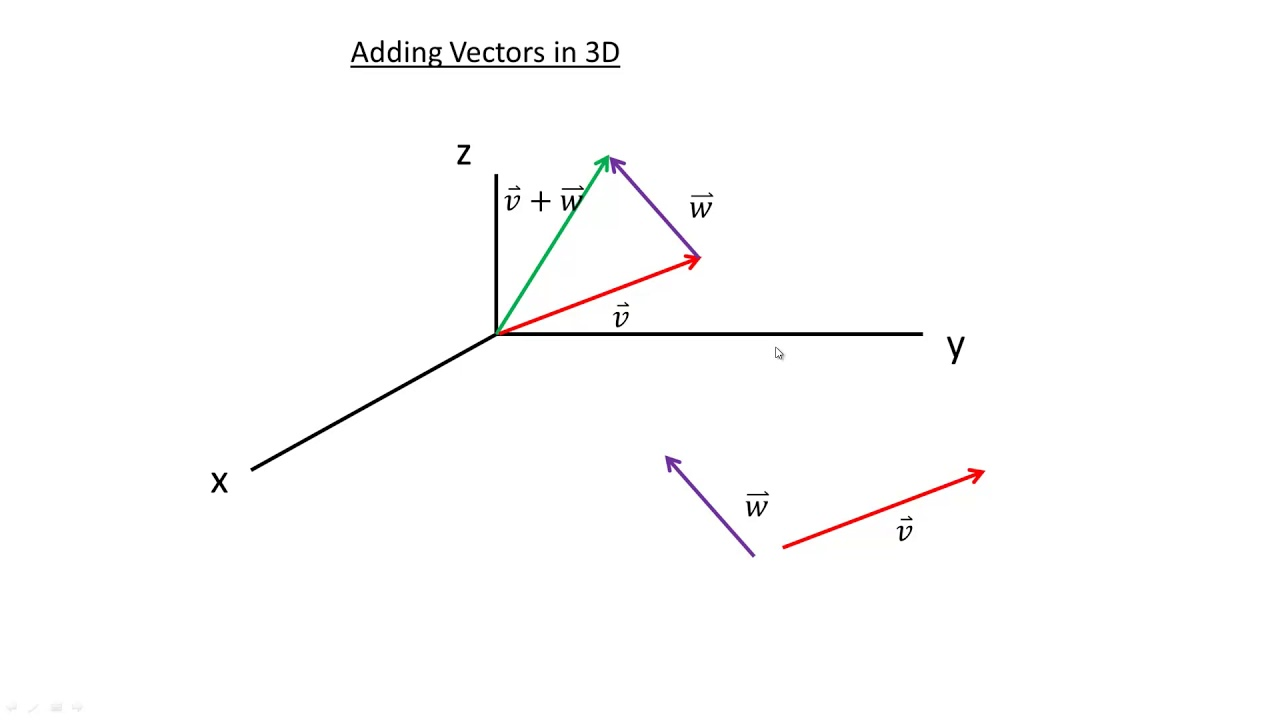
\includegraphics[width=\linewidth]{images/addingvectors.jpg}
\subsubsection{Scaling}
Algebraically, scale each component individually
$$
\lambda \left(
    \begin{array}{c}  
         x \\
         y \\
         z
    \end{array}
    \right) = \left(
    \begin{array}{c}  
         \lambda x \\
         \lambda y \\
         \lambda z
    \end{array}
    \right)
$$

Geometrically, if you scale a vector by a positive real number, direction stays the same but length is changed. \\
\begin{center}
    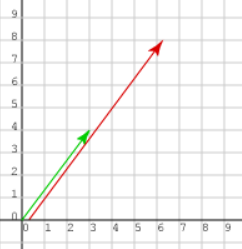
\includegraphics[width=0.3\linewidth]{images/scalingvector.png}
\end{center}
If scaled by a negative number, the direction flips (and length changes too).

\subsubsection{Length}
Algebraically, length is calculated using Pythagoras' theorem.
$$\left| \left(
    \begin{array}{c}  
         x \\
          y \\
          z
    \end{array}
    \right) \right| = \sqrt{x^2 + y^2 + z^2}
    $$

\subsubsection{Dot Product}
Dot product takes 2 vectors and outputs a single real number.
$$\left(
    \begin{array}{c}  
         x_1 \\
         y_1 \\
         z_1
    \end{array}
    \right) \cdot \left(
    \begin{array}{c}  
         x_2 \\
         y_2 \\
         z_2
    \end{array}
    \right) = x_1 x_2 + y_1 y_2 + z_1 z_2 
$$
Geometrically, dot product is a measure of how similar the direction of the 2 vectors are.
$$\vec{a} \cdot \vec{b} = |\vec{a}| |\vec{b}| \cos \theta $$
where $\theta$ is the angle between the 2 vectors.\\[10pt]
The dot product is used to define 
\begin{itemize}
    \item Work Done $W.(D) = \int \vec{F} \cdot d\vec{r}$
    \item Magnetic Flux $\Phi = \int \vec{B} \cdot d\vec{A}$
\end{itemize}

\subsubsection{Cross Product}
Cross product takes 2 vectors and outputs another vector.
$$\left(
    \begin{array}{c}  
         x_1 \\
         y_1 \\
         z_1
    \end{array}
    \right) \times \left(
    \begin{array}{c}  
         x_2 \\
         y_2 \\
         z_2
    \end{array} 
    \right) = \left(
    \begin{array}{c}  
         y_1 z_2 - z_1 y_2 \\
         z_1 x_2 - x_1 z_2 \\
         x_1 y_2 - y_1 x_2
    \end{array}
    \right)
$$

Geometrically, the length of the cross product is the area of the parallelogram. The direction of the cross product is perpendicular (following right hand rule). \\
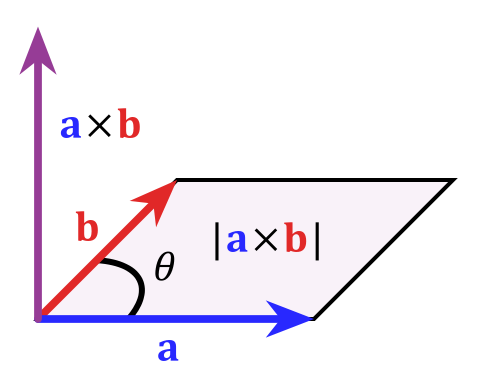
\includegraphics[width=0.49\linewidth]{images/crossproduct.png}
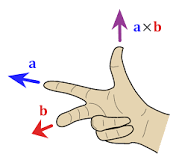
\includegraphics[width=0.49\linewidth]{images/crossproduct2.png}\\
The cross product is used to define 
\begin{itemize}
    \item Torque $\vec{\tau} = \vec{r} \times \vec{F}$
    \item Angular Momentum $\vec{L} = \vec{r} \times \vec{p}$
    \item Lorentz Force $\vec{F} = q(\vec{E} + \vec{v}\times \vec{B})$
    \item Poynting Vector $\vec{S}=\frac{1}{\mu_0} \vec{E} \times \vec{B}$
\end{itemize}

\subsubsection{Derivatives}
Also done component wise
$$\frac{d\vec{r}}{dt} = \frac{d}{dt}\left(
    \begin{array}{c}  
         x \\
         y \\
         z
    \end{array} 
    \right) = \left(
    \begin{array}{c}  
         dx/dt \\
         dy/dt \\
         dz/dt
    \end{array} 
    \right)
$$

\subsection{Exercises}
\begin{samepage}
SJPO 2015 General Round Q11: A force $\vec{F} = \vec{F}_1 + \vec{F}_2$ can be decomposed as the sum of 2 vectors $\vec{F}_1$ and $\vec{F}_2$. Only the magnitude of $\vec{F}_1$ and the direction of $\vec{F}_2$ are known. Which of the following is the most accurate statement?
\begin{itemize}
\item[](A) Only one combination of $\vec{F}_1$ and $\vec{F}_2$ exists.
\item[](B) There exists exactly two combinations of $\vec{F}_1$ and $\vec{F}_2$.
\item[](C) There exists infinite combinations of $\vec{F}_1$ and $\vec{F}_2$.
\item[](D) At least three combinations of $\vec{F}_1$ and $\vec{F}_2$ exist but the total number of combinations is finite.
\item[](E) Only one or two combinations of $\vec{F}_1$ and $\vec{F}_2$ exist.
\end{itemize}
Ans: E
\end{samepage}
\begin{samepage}
\subsubsection{SJPO 2016 General Round Q21}
Initially, a $1\mathrm{~kg}$ box was sliding on frictionless surface at a constant velocity of $4\mathrm{~ms}^{-1}$ in the $\mathrm{x}$ direction. A constant force of $1\mathrm{~N}$ was applied on the box in a fixed direction for a time duration of $5\mathrm{~s}$. After $5\mathrm{~s}$ the speed of the box is $3\mathrm{~ms}^{-1}$. What is the magnitude of the change in momentum of the box?
\begin{itemize}
\item[](A) $1 \mathrm{kgms}^{-1}$
\item[](B) $2 \mathrm{kgms}^{-1}$
\item[](C) $3 \mathrm{kgms}^{-1}$
\item[](D) $4 \mathrm{kgms}^{-1}$
\item[](E) $5 \mathrm{kgms}^{-1}$
\end{itemize}
Ans: E \\[10pt]
Extra: What are the possible directions of the applied force? 
\end{samepage}
\newpage
\section{Physics: Dynamics and Projectile Motion}

The following quantities are scalars (real numbers)
\begin{itemize}
    \item mass $m$
    \item speed $|\vec{v}|$
    \item kinetic energy $E = \frac{1}{2} m|\vec{v}|^2$
    \item potential energy $U$
\end{itemize}
\leavevmode \\
The following quantities are vectors
\begin{itemize}
    \item position $\vec{r}(t)$
    \item velocity $\vec{v}(t) \equiv \frac{d\vec{r}}{dt}$
    \item acceleration $\vec{a}(t) \equiv \frac{d^2\vec{r}}{dt^2}$
    \item force $\vec{F}(t)$
    \item momentum $\vec{p}(t) \equiv m\vec{v}(t)$
\end{itemize}
\leavevmode \\
Newton's 2nd law
$$\vec{F}_{\text{net}} = \frac{d\vec{p}}{dt}$$
Newton's 3rd law 
$$\vec{F}_{\text{A on B}} = -\vec{F}_{\text{B on A}}$$

\subsection{Projectile Motion}
\begin{align}
\vec{F}_{\text{net}} &= m \vec{a} \\
\Rightarrow \left(
    \begin{array}{c}  
         0 \\
         -mg \\
         0
    \end{array} 
    \right) &= m \left(
    \begin{array}{c}  
         d^2x/dt^2 \\
         d^2y/dt^2 \\
         d^2z/dt^2
    \end{array} 
    \right)
\end{align}
Integrating twice with respect to time $t$,
\begin{align}
    \left(
    \begin{array}{c}  
         x(t) \\
         y(t) \\
         z(t)
    \end{array} 
    \right) = \left(
    \begin{array}{c}  
          {u}_x t + {r_0}_x\\
         -\frac{1}{2}gt^2 + {u}_y t + {r_0}_y\\
          {u}_z t + {r_0}_z
    \end{array} 
    \right)
\end{align}
We need to know the initial position $\vec{r}_0 \equiv \vec{r}(t=0)$ and initial velocity $\vec{u} \equiv \vec{v}(t=0)$. For example, 
\begin{align}
    \vec{r}(t=0) &= \left(
    \begin{array}{c}  
         0 \\
         0 \\
         0
    \end{array} 
    \right) \\
    \vec{v}(t=0) &= \left(
    \begin{array}{c}  
         u \cos \theta \\
         u \sin \theta \\
         0
    \end{array} 
    \right)
\end{align}   
Then that gives us the path of the projectile with respect to time
\begin{align}
    x(t) &= u \cos \theta\ t \label{eq:xt} \\
    y(t) &= u \sin \theta\ t - \frac{1}{2} gt^2 \\
    z(t) &= 0
\end{align}
This is also known as a parametric curve, with time $t$ being the parameter. Every value of $t$ gives us a point in space $(x(t),y(t),z(t))$. 

\subsubsection{From parametric to $y(x)$}
If we want to convert parametric curve into a formula for the graph $y(x)$, then we need to invert Equation \ref{eq:xt} to yield $$t(x) = {\frac{x}{u \cos \theta}}$$
Substituting $t(x)$ into $y(t)$ gives us $y(x)$
\begin{align}
    y(x) &= \tan \theta\ x - \frac{g}{2u^2 \cos^2 \theta} x^2
\end{align}
\subsubsection{Finding Range}
There are 2 solutions to $y(x) = 0$: the starting one being $x_{\text{start}}=0$. The other is 
$$x_{\text{end}} = \frac{2u^2}{g} \sin \theta \cos \theta = \frac{u^2}{g} \sin 2\theta$$

We now have range as a function of angle $x_{\text{end}}(\theta)$. We can differentiate this with respect to $\theta$ and set the derivative $dx_{\text{end}}/d\theta = 0$ to find the maximum range. Strictly speaking, we have to check the second derivative too.
% \subsubsection{Region of Reachability}
\subsection{Exercises}
Region of Reachability\\
Hitting a slope\\
Starting from a height \\
Minimum velocity to cross a wall (spot)\\
(ODE) With air resistance
\section{Math: Differential Equations}
When we studied $F(t)=ma(t)$, we noted that as long as we know the function $F(t)$, we can find $a(t)$ and integrate twice to obtain $x(t)$. However, in most systems, $F(t)$ depends on $x(t)$ or $v(t) \equiv \dot{x}(t)$. Examples include 
\begin{itemize}
    \item Spring Mass $F(x(t)) = -kx(t)$
    \item Gravitation $F(\vec{r}(t)) = -\frac{GMm}{|\vec{r(t)}|^2} \hat{r}$
    \item Drag $F(v(t)) = \frac{1}{2} \rho v(t)^2 C_D A$
    \item Lorentz Force $\vec{F} = q(\vec{E} + \vec{v} \times \vec{B})$
\end{itemize}
In these scenarios, we can no longer simply "integrate twice" since we hit a circular dependency. To resolve this, we need to solve the "differential equation". Differential equations are very common in physics. If you solve the Navier-Stokes Differential Equation, you earn a million dollars.
\subsection{What is a Differential Equation?}
When we first learned the quadratic equation, we were looking for \textbf{values} of $x$ that satisfy $$ax^2 + bx + c = 0$$  We can find 2 complex \textbf{solutions} to this \textbf{algebraic} equation
$$x = \frac{-b - \sqrt{b^2 - 4ac}}{2a} \quad \text{or}\quad x = \frac{-b + \sqrt{b^2 - 4ac}}{2a}$$
In \textbf{differential} equations, we are looking for \textbf{functions} $y(x)$ that satisfy (for example)
$$\frac{dy}{dx} = y$$
In this example, $y(x) = e^x$ works! Substitute it into the above to check that $\text{LHS} = \text{RHS}$. In fact, one can check that any multiple of $e^x$ works too! So $y(x) = A e^x$ for any arbitrary constant $A$ is a solution. To determine $A$, we need to know the "initial condition" $y(0) = A$.
\\[10pt]
Let's try another example, find the function $y(x)$ that satisfies 
$$\frac{dy}{dx} = 5y$$ with initial condition $\left. \frac{dy}{dx} \right|_{x=0} = 10$\\
Solution: $y(x) = 2e^{5x}$
\subsubsection{Physics: RC circuit} 
Find $q(t)$ that satisfies the following ($R,C$ are constants).
$$\frac{dq}{dt} = -\frac{q}{RC}$$ with initial condition $q(t=0) = q_0$. \\Answer: $q(t) = q_0 \exp (-t/RC)$ \\[10pt]
What if the initial condition was $I(t=0) := \left. \frac{dq}{dt} \right|_{t=0} = I_0$ instead? \\ Answer: $q(t) = {I_0 RC} \exp (-t/RC)$\\[10pt]

\subsection{2nd Order Differential Equations}
In polynomial equations, the largest power $x^n$ is the degree $n$ of the polynomial. In differential equations, the highest derivative $\frac{d^n y}{dx^n}$ is the order of the differential equation. In this section, we cover a very common class of 2nd order differential equations
$$\frac{d^2 y}{dx^2} = -\omega^2 y$$
which has solution
$$y(x) = A\sin(\omega x + \phi)$$
\subsubsection{Derivation by Layman Arguments}
$\sin x$ and $\cos x$ are the only (proof involves linear algebra) functions that when differentiated twice, pick up a negative sign. We can afford to put a constant $\phi$ in the parameter of $\sin$, since constants vanish when differentiated. 

\subsubsection{Derivation using Complex Exponential }
\begin{align}
    \frac{d^2 y}{ dx^2} = A y     \label{eq:shm}
\end{align}
where $-\infty < A < \infty$ is a real constant.\\[10pt]
Solution: $$y=y_0 \exp(\sqrt{A}x)$$ 
Question: What happens if $A < 0$? \\
Answer: $\sqrt{A}$ is complex! To be more precise, if $A=-\omega^2$ for a positive real number $\omega$, then 
$$y=y_0 \exp(\pm i \omega x)$$
are 2 valid solutions.

\textbf{A word on linear differential equation: } Equation \ref{eq:shm} is said to be linear, because if I have 2 solutions $f(x)$ and $g(x)$, then adding them together or scaling them is still a valid solution.
\begin{align}
    \text{Given } \frac{d^2 f}{ dx^2} &= A f(x)\\
    \text{And } \frac{d^2 g}{ dx^2} &= A g(x) \\
    y(x) &= f(x) + g(x)\text{ is a solution too }\\
    \text{Goal: Show } \frac{d^2y}{dx^2} & = Ay(x)\\
    \text{Proof: LHS} &= \frac{d^2}{dx^2} [f(x)+g(x)] \\
    &= \frac{d^2 f}{dx^2} + \frac{d^2 g}{dx^2} \\ 
    &= A f(x) + A g(x) \\
    &= A [f(x) + g(x)] \\
    &= \text{RHS}
\end{align}

Examples of Linear Differential Equations:
\begin{itemize}
    \item Simple Harmonic Motion
    \item RLC Circuits (linear components)
    \item (Linear) Wave Equation
    \item Schrodinger equation (Quantum Mechanics)
    \item Maxwell's Equation (Electromagnetism)
\end{itemize}
\leavevmode \\
Since $$y_+(x)=y_0 \exp(+ i \omega x)$$ and $$y_-(x) = y_0 \exp(- i \omega x)$$ are 2 solutions to the \textbf{linear} DE $$\frac{d^2 f}{ dx^2} = A f(x)$$
any linear combination of them is a valid solution.

$$y(x) = C \exp(+i\omega x) + D \exp(-i \omega x)$$
where $C,D$ are arbitrary complex constants.

\textbf{But what is a complex exponential? } Euler's formula: 
$$e^{i\theta} = \cos \theta + i \sin \theta$$
Some say it's just a mathematical trick, since "our system doesn't involve complex numbers". It gets philosophical. Richard Feynman famously said: "Shut up and calculate". \\[10pt]
So we want our solution $y(x)$ to be real, i.e. $\text{Im }[y(x)] = 0$. So that necessitates that $C^* = D$ and so the general solution is 
\begin{align}
    y(x) &= C \exp(+i\omega x) + C^* \exp(-i\omega x)\\
    &\ \ |\quad \text{Polar Form: }C := |C| \exp(i \phi) \\
    &= |C| \text{Re}[\exp(+i (\omega x + \phi))] \\
    &= |C| \cos (\omega x + \phi)
\end{align}
which is the general solution we heuristically arrived at previously. The complex exponential solution adds more rigour to the claim that "this is the most general solution possible".

\subsubsection{Simple Harmonic Motion}

There are a lot of ways Simple Harmonic Motion (SHM) can appear, but one thing that is universal is that the equations of motion always simplify (usually after some approximations) to the form 
\begin{align}
    \frac{d^2 y}{dt^2} &= -\omega^2 y(t) \\
    y(t) &= A \sin (\omega t + \phi)
\end{align}
where $\omega = 2\pi/T$ will turn out to be the angular frequency of the oscillation, $T$ being the period of oscillation. \\[10pt]
Side note: The $\phi$ accounts for the $\cos$ solution by R-formula $a \sin \theta + b \cos \theta = \sqrt{a^2 + b^2} \sin(\theta + \arctan \left(\frac{b}{a}\right))$



\subsection{Physics Examples/Exercises}
\subsubsection{Spring Mass}
A mass $m$ lies on a frictionless table, attached to an unstretched spring with spring constant $k$. The other end of the spring is fixed to a wall. The mass is displaced from it's equilibrium position by $x_0$ (in a direction perpendicular to the wall) and released. Find the amplitude and period of oscillation.\\[10pt]
Hooke's Law: The restoring force $F$ of a spring stretched by $\vec{r}$ is $F(\vec{r}) = -k\vec{r}$.\\[10pt]
Extra: Find the period of oscillation of a mass $m$ hung vertically on a spring with spring constant $k$ in a gravitational field strength $g$.

\subsubsection{Spring Mass (with a Push)}
Same as the above, mass $m$ on frictioness table attached to spring with spring constant $k$ displaced by $x_0$. But this time, instead of a release, it is pushed, giving the mass an initial speed $v_0$ (toward the point of equilibrium). Find the new amplitude of oscillation.\\[10pt]
This question emphasizes the initial conditions of a differential equation.

\subsubsection{Pendulum}
A mass $m$ is hung by an inextensible string of length $l$ in a gravitational field strength $g$. It is displaced by a small angular displacement $\theta_0$ and released. Find the amplitude and period of oscillation.

\section{Physics: Newtonian Mechanics}
Newton's Three Laws
\subsection{}
\subsection{Momentum \& Impulse}
Change in a particle's momentum is equal to the impulse it experiences. \\[10pt]
Newton's 2nd law: Let $\vec{F}(t)$ be the net force on a particle, then
$$\vec{F}(t) = \frac{d\vec{p}}{dt}$$
Let's focus on one component of the vector equation (say $F_x, p_x$)
$$F_x(t) = \frac{dp_x}{dt}$$
Integrating both sides wrt time $t$ from $t=t_A$ to $t=t_B$ yields

\begin{align}
    \int_{t_A}^{t_B} F_x(t) dt &= \int_{t_A}^{t_B} \frac{dp_x}{dt} dt \\
    \int_{t_A}^{t_B} F_x(t) dt &= \int_{p_x(t_A)}^{p_x(t_B)} dp_x \\
    &= p_x(t_B) - p_x(t_A) \\
    &= \Delta p_x
\end{align}
If a particle experiences a force $\vec{F}(t)$ over a time period $t_A$ to $t_B$, it's ($x$-component of) momentum will change by $\Delta p_x = \int_{t_A}^{t_B} F_x(t) dt$.\\[10pt]
This is true for each component $x,y,z$ so actually it is a vector equation 
$$\Delta \vec{p} = \int_{t_A}^{t_B} \vec{F}(t) dt$$
The quantity on the right hand side is called impulse.


\section{Kinetic Energy \& Work}


\end{document}
